% Options for packages loaded elsewhere
% Options for packages loaded elsewhere
\PassOptionsToPackage{unicode}{hyperref}
\PassOptionsToPackage{hyphens}{url}
\PassOptionsToPackage{dvipsnames,svgnames,x11names}{xcolor}
%
\documentclass[
  letterpaper,
  DIV=11,
  numbers=noendperiod]{scrartcl}
\usepackage{xcolor}
\usepackage{amsmath,amssymb}
\setcounter{secnumdepth}{-\maxdimen} % remove section numbering
\usepackage{iftex}
\ifPDFTeX
  \usepackage[T1]{fontenc}
  \usepackage[utf8]{inputenc}
  \usepackage{textcomp} % provide euro and other symbols
\else % if luatex or xetex
  \usepackage{unicode-math} % this also loads fontspec
  \defaultfontfeatures{Scale=MatchLowercase}
  \defaultfontfeatures[\rmfamily]{Ligatures=TeX,Scale=1}
\fi
\usepackage{lmodern}
\ifPDFTeX\else
  % xetex/luatex font selection
\fi
% Use upquote if available, for straight quotes in verbatim environments
\IfFileExists{upquote.sty}{\usepackage{upquote}}{}
\IfFileExists{microtype.sty}{% use microtype if available
  \usepackage[]{microtype}
  \UseMicrotypeSet[protrusion]{basicmath} % disable protrusion for tt fonts
}{}
\makeatletter
\@ifundefined{KOMAClassName}{% if non-KOMA class
  \IfFileExists{parskip.sty}{%
    \usepackage{parskip}
  }{% else
    \setlength{\parindent}{0pt}
    \setlength{\parskip}{6pt plus 2pt minus 1pt}}
}{% if KOMA class
  \KOMAoptions{parskip=half}}
\makeatother
% Make \paragraph and \subparagraph free-standing
\makeatletter
\ifx\paragraph\undefined\else
  \let\oldparagraph\paragraph
  \renewcommand{\paragraph}{
    \@ifstar
      \xxxParagraphStar
      \xxxParagraphNoStar
  }
  \newcommand{\xxxParagraphStar}[1]{\oldparagraph*{#1}\mbox{}}
  \newcommand{\xxxParagraphNoStar}[1]{\oldparagraph{#1}\mbox{}}
\fi
\ifx\subparagraph\undefined\else
  \let\oldsubparagraph\subparagraph
  \renewcommand{\subparagraph}{
    \@ifstar
      \xxxSubParagraphStar
      \xxxSubParagraphNoStar
  }
  \newcommand{\xxxSubParagraphStar}[1]{\oldsubparagraph*{#1}\mbox{}}
  \newcommand{\xxxSubParagraphNoStar}[1]{\oldsubparagraph{#1}\mbox{}}
\fi
\makeatother


\usepackage{longtable,booktabs,array}
\usepackage{calc} % for calculating minipage widths
% Correct order of tables after \paragraph or \subparagraph
\usepackage{etoolbox}
\makeatletter
\patchcmd\longtable{\par}{\if@noskipsec\mbox{}\fi\par}{}{}
\makeatother
% Allow footnotes in longtable head/foot
\IfFileExists{footnotehyper.sty}{\usepackage{footnotehyper}}{\usepackage{footnote}}
\makesavenoteenv{longtable}
\usepackage{graphicx}
\makeatletter
\newsavebox\pandoc@box
\newcommand*\pandocbounded[1]{% scales image to fit in text height/width
  \sbox\pandoc@box{#1}%
  \Gscale@div\@tempa{\textheight}{\dimexpr\ht\pandoc@box+\dp\pandoc@box\relax}%
  \Gscale@div\@tempb{\linewidth}{\wd\pandoc@box}%
  \ifdim\@tempb\p@<\@tempa\p@\let\@tempa\@tempb\fi% select the smaller of both
  \ifdim\@tempa\p@<\p@\scalebox{\@tempa}{\usebox\pandoc@box}%
  \else\usebox{\pandoc@box}%
  \fi%
}
% Set default figure placement to htbp
\def\fps@figure{htbp}
\makeatother





\setlength{\emergencystretch}{3em} % prevent overfull lines

\providecommand{\tightlist}{%
  \setlength{\itemsep}{0pt}\setlength{\parskip}{0pt}}



 


\KOMAoption{captions}{tableheading}
\makeatletter
\@ifpackageloaded{caption}{}{\usepackage{caption}}
\AtBeginDocument{%
\ifdefined\contentsname
  \renewcommand*\contentsname{Table of contents}
\else
  \newcommand\contentsname{Table of contents}
\fi
\ifdefined\listfigurename
  \renewcommand*\listfigurename{List of Figures}
\else
  \newcommand\listfigurename{List of Figures}
\fi
\ifdefined\listtablename
  \renewcommand*\listtablename{List of Tables}
\else
  \newcommand\listtablename{List of Tables}
\fi
\ifdefined\figurename
  \renewcommand*\figurename{Figure}
\else
  \newcommand\figurename{Figure}
\fi
\ifdefined\tablename
  \renewcommand*\tablename{Table}
\else
  \newcommand\tablename{Table}
\fi
}
\@ifpackageloaded{float}{}{\usepackage{float}}
\floatstyle{ruled}
\@ifundefined{c@chapter}{\newfloat{codelisting}{h}{lop}}{\newfloat{codelisting}{h}{lop}[chapter]}
\floatname{codelisting}{Listing}
\newcommand*\listoflistings{\listof{codelisting}{List of Listings}}
\makeatother
\makeatletter
\makeatother
\makeatletter
\@ifpackageloaded{caption}{}{\usepackage{caption}}
\@ifpackageloaded{subcaption}{}{\usepackage{subcaption}}
\makeatother
\usepackage{bookmark}
\IfFileExists{xurl.sty}{\usepackage{xurl}}{} % add URL line breaks if available
\urlstyle{same}
\hypersetup{
  pdftitle={Spatial Inequalities in Educational Infrastructure: Bayesian Hierarchical Modelling of School Availability Across North Borneo},
  pdfauthor={Alvin Bong},
  colorlinks=true,
  linkcolor={blue},
  filecolor={Maroon},
  citecolor={Blue},
  urlcolor={Blue},
  pdfcreator={LaTeX via pandoc}}


\title{Spatial Inequalities in Educational Infrastructure: Bayesian
Hierarchical Modelling of School Availability Across North Borneo}
\author{Alvin Bong}
\date{}
\begin{document}
\maketitle
\begin{abstract}
Understanding the spatial distribution of educational infrastructure is
essential for ensuring equitable access to schooling. This study
examines regional disparities in school availability across Brunei and
the neighboring Malaysian states of Sarawak and Sabah, with a focus on
identifying potential underserved areas. First, exploratory data
analysis (EDA) was conducted to compare school counts and
student-teacher ratios at the district level across the three regions.
The core analysis employs Standardized Incidence Ratio (SIR) and
Bayesian spatial Poisson model using Integrated Nested Laplace
Approximation (INLA) to estimate the relative abundance of schools
across Brunei's districts, adjusting for expected counts based on
population, region size and socioeconomic indicator (house price +
partially simulated). Spatially structured and unstructured random
effects were incorporated to account for latent spatial processes.
Posterior estimates identified districts with significantly lower school
availability than the national baseline, supporting future policy
planning and school placement.
\end{abstract}


\subsection{Introduction}\label{introduction}

Education is a foundational pillar of national development and its
people, influencing social well-being, economic growth, and long-term
sustainability. The global significance of education is recognized in
Sustainable Development Goal 4, which promotes inclusive and equitable
quality education for all {[}1{]}. Nationally, Brunei Darussalam's
national vision, Wawasan Brunei 2035, positions education as a
cornerstone of the country's long-term development goals. Ensuring
equitable access to education through sufficient infrastructure, fair
resource distribution, and balanced student--teacher ratios is critical
to delivering quality learning experiences.

While several studies have examined general aspects of education in
Brunei, there have been limited studies based on quantitative spatial
methods, with only one examining the spatial distribution and hotspots
of schools. This project aims to addresses that gap by first conducting
a comparative analysis of school availability and student--teacher
ratios across Brunei's districts, with additional context from
neighboring Malaysian states, Sarawak and Sabah.

Next, Standardized Incidence Ratios (SIR) and Bayesian hierarchical
models are used to identify adminstrative regions in Brunei where school
availability falls significantly below the national baseline, supporting
future policy planning and school placements.

\subsection{Data}\label{data}

This study focuses exclusively on government primary and secondary
schools, as these institutions serve as the main access points to
education for most youth. The school dataset from 2018 was used as it is
the most recent year for which disaggregated school-level data is
available in Brunei. Although more recent statistics exist, they are
published only in summary form.

Population data is drawn from the 2021 national census, the most recent
census available in Brunei, despite the mismatch in years with the
school dataset. Brunei conducts its national census every ten years,
making the 2021 data the best option for population estimates.

The following key data variables were used: school counts,
administrative boundary data, population, student--teacher ratios, and
house prices. These datasets were cleaned, wrangled, and merged
primarily using left\_join() and rbind(), with further details provided
below.

\subsubsection{Brunei}\label{brunei}

Data on school locations, student--teacher ratios, administrative
boundaries, and population were sourced from the \texttt{bruneimap} R
package. The school dataset \texttt{sch\_sf} includes georeferenced
point data for each institution. For our areal analysis, schools were
aggregated by district and mukim (finer administrative level). Despite
composing of only four districts, district-level aggregation was used
for broader comparisons (student--teacher ratios and school counts) to
match the size of available administrative resolution in Malaysian data.
Mukims (\(N = 39\)), which provide finer geographic resolution, were
instead used for the Bayesian spatial analysis of school availability in
Brunei.

To incorporate a socioeconomic indicator, we used median house prices
derived from approximately 30,000 property listings spanning 1993--2025.
These were calculated at the mukim level and included as a covariate in
the Bayesian model. In cases where house price data were missing, values
were imputed using predictions from an INLA-based Gaussian model. Manual
imputations based on local knowledge were initially tested, but the
INLA-predicted values were ultimately adopted, as both methods produced
similar model outcomes. Given the nature of the data, house prices were
treated as partially simulated estimates and may not fully reflect
actual market values.

\subsubsection{Malaysia}\label{malaysia}

Malaysian data variables were sourced from the national open data portal
{[}data.gov.my{]}, and include district-level school counts and
population estimates for the states of Sarawak and Sabah. Administrative
boundary (districts) were obtained via the \texttt{geomdata} R package,
as OpenStreetMap (\texttt{osmdata}) does not provide required
administrative divisions level.

Some inconsistencies were found between school data and adminstrative
boundaries, particularly in areas where older districts had been
subdivided into newer ones. In these cases, school counts were available
only for the original (larger) districts. To ensure consistency, we
excluded the newer subdivisions and manually reassigned schools in the
affected areas to the nearest valid district.

\subsection{Method}\label{sec-method}

Exploratory data anlysis using Clorepath maps for schools count, by area
(usingst\_area) studnet teacher ratio

Neighbour type

POisson INLA hierarchical model

covariates: house price as socio economic index

Spatial Poisson model Justify offset (population) Explain fixed and
random effects Introduce INLA + BYM

\subsection{Results}\label{sec-results}

\pandocbounded{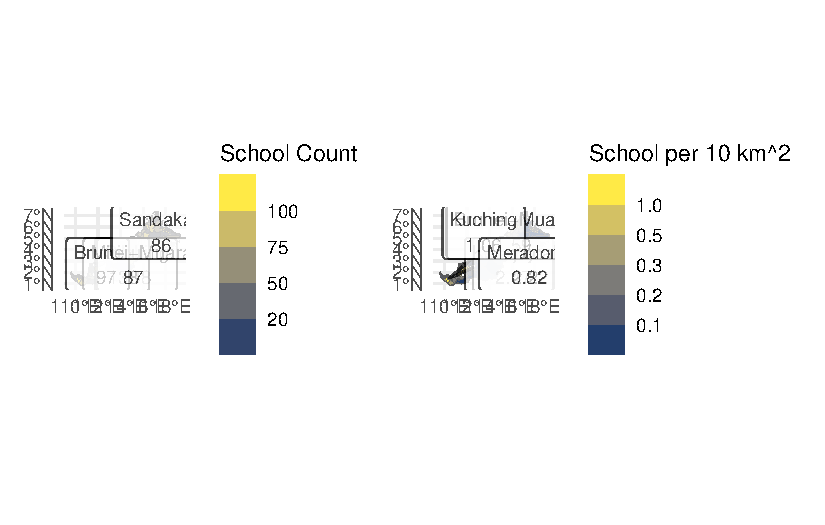
\includegraphics[keepaspectratio]{index_files/figure-pdf/unnamed-chunk-1-1.pdf}}

\pandocbounded{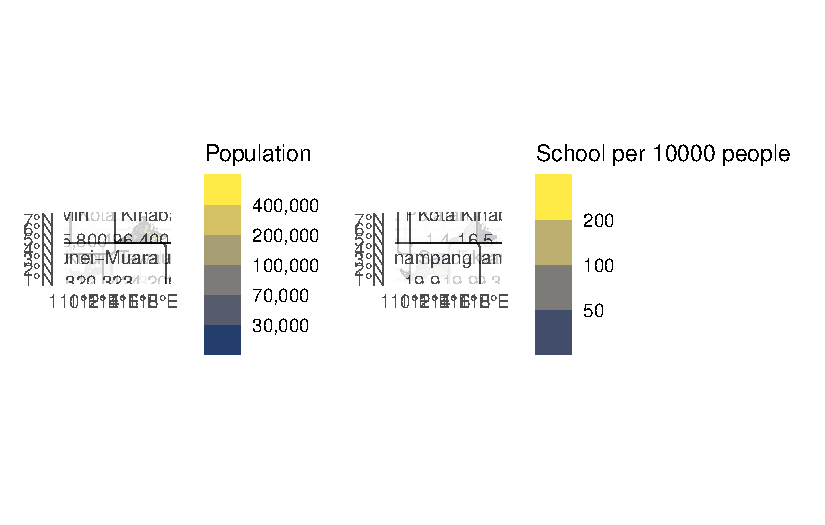
\includegraphics[keepaspectratio]{index_files/figure-pdf/unnamed-chunk-1-2.pdf}}

\begin{itemize}
\tightlist
\item
  School count quite similar, more in main city
\end{itemize}

\begin{verbatim}
character(0)
\end{verbatim}

\begin{verbatim}
[1] "Matu"     "Pakan"    "Selangau"
\end{verbatim}

\begin{verbatim}
character(0)
\end{verbatim}

\begin{verbatim}
[1] "Matu"     "Pakan"    "Selangau"
\end{verbatim}

\pandocbounded{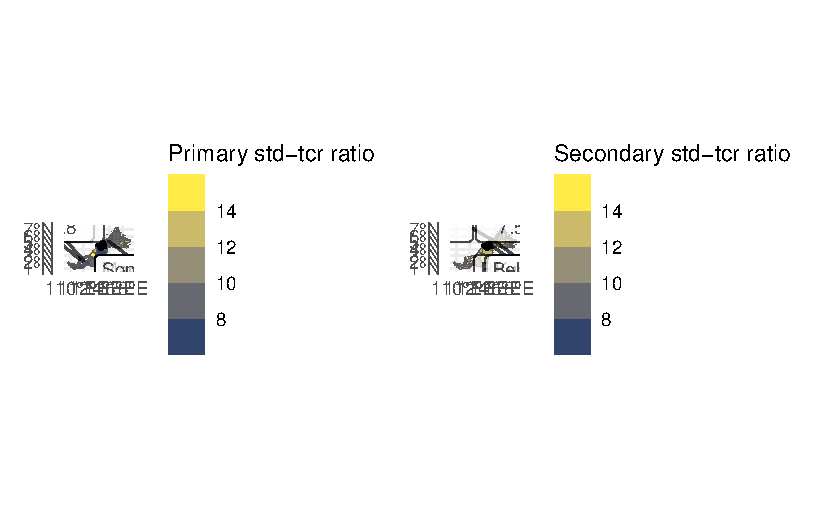
\includegraphics[keepaspectratio]{index_files/figure-pdf/unnamed-chunk-2-1.pdf}}

\begin{itemize}
\tightlist
\item
  studnet teacher ratio, primary simiilar other than dense city (miri,
  kuching, kota kinabalu), but brunei has lesser secondary std-tcr{]}
\end{itemize}

\subsubsection{Model}\label{model}

\pandocbounded{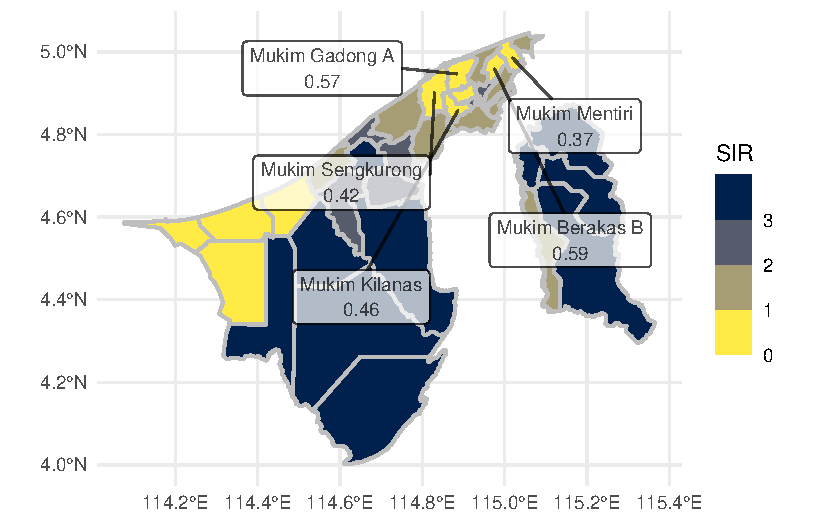
\includegraphics[keepaspectratio]{index_files/figure-pdf/unnamed-chunk-4-1.pdf}}

\begin{itemize}
\tightlist
\item
  There are significantly fewer schools in Mukim xxx
\end{itemize}

\pandocbounded{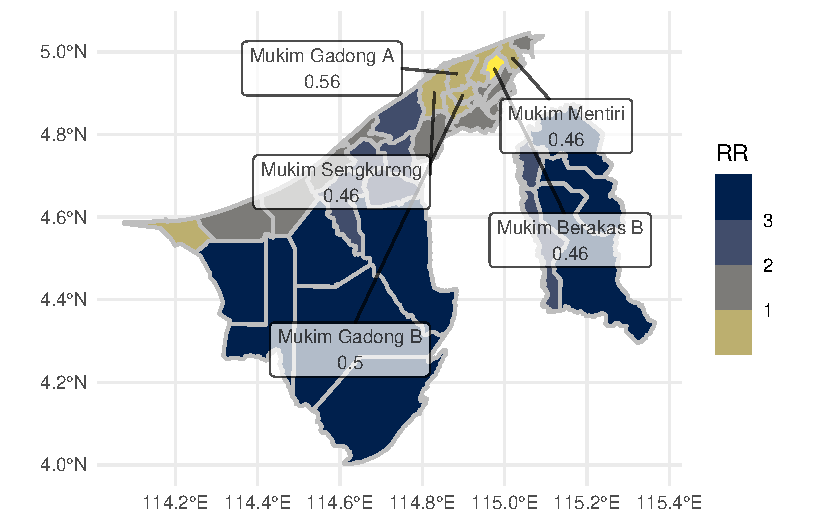
\includegraphics[keepaspectratio]{index_files/figure-pdf/unnamed-chunk-6-1.pdf}}

\pandocbounded{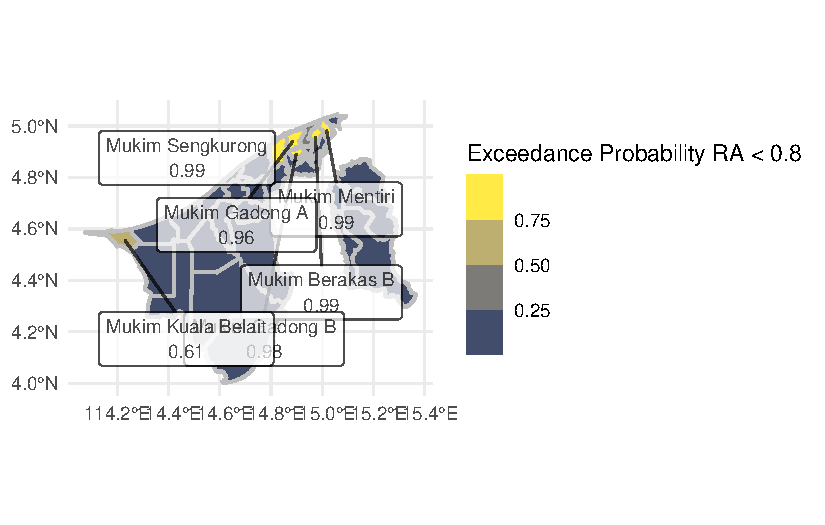
\includegraphics[keepaspectratio]{index_files/figure-pdf/unnamed-chunk-7-1.pdf}}

\begin{itemize}
\tightlist
\item
  Coefficient , sginificance
\end{itemize}

\subsection{Discussion \& Limitation}\label{discussion-limitation}

There are significantly fewer schools in Mukim xxx, when explored, its
not forested area. Housing region, some may be newer nieghbourhood so..
good idea for mroe schools there, nearer from home, less transportation
cost, environmental, time.

Given that Brunei has higher PISA scores than Malaysia, it would be
interesting to explore whether accessibility may be a potential factor.
/ Malaysia has more population than Brunei, how does the school compare

Limitation: only public schools, to consider private schools age groups,
2018 data, school types, some simulation in housing price, house price
is listing price (only a proxy for market values), may deviate from
actual sales price due to negotian dynamics and other factors \#\#
Conclusions \{\#sec-conc\}

\begin{itemize}
\tightlist
\item
  School count quite similar, more in main city
\item
  studnet teacher ratio, primary simiilar other than dense city (miri,
  kuching, kota kinabalu), but brunei has lesser secondary std-tcr
\item
  There are significantly fewer schools in Mukim xxx
\end{itemize}

\subsection*{References}\label{references}
\addcontentsline{toc}{subsection}{References}

\phantomsection\label{refs}




\end{document}
